\documentclass[titlepage]{article}
\usepackage[margin=0.5in]{geometry}
\usepackage{graphicx}
\usepackage{minted}

\title{VLSI \\Assignment 3 Annexure}
\author{Priyank Lohariwal\\BCSE IV\\Roll-001710501055}
\date{}

\begin{document}
    {\maketitle}

    \section{Describtion}
    \begin{itemize}
        \item Design a 4x16 decoder by only behavioral modelling 
        \begin{itemize}
            \item  by using function of 2x4 decoders only
            \item  by using procedures of 2x4 decoders only
        \end{itemize}
    \end{itemize}

    \section{Block Diagram} 
    \begin{figure}[!ht]
        \centering
        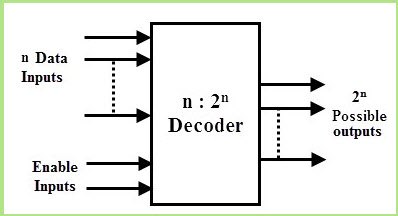
\includegraphics{./figures/Decoder-Block-Diagram.jpg}
        \caption{Decoder block diagram}
    \end{figure}


    \section{Truth Table}
    \begin{tabular}{| c | c |}
        \hline
        X(3 - 0) & Y(15 - 0) \\
        \hline
        0000 & 0000000000000001 \\
        0001 & 0000000000000010 \\
        0010 & 0000000000000100 \\
        0011 & 0000000000001000 \\
        0100 & 0000000000010000 \\
        0101 & 0000000000100000 \\
        0110 & 0000000001000000 \\
        0111 & 0000000010000000 \\
        1000 & 0000000100000000 \\
        1001 & 0000001000000000 \\
        1010 & 0000010000000000 \\
        1011 & 0000100000000000 \\
        1100 & 0001000000000000 \\
        1101 & 0010000000000000 \\
        1110 & 0100000000000000 \\
        1111 & 1000000000000000 \\
        \hline
    \end{tabular}
    \section{Circuit Diagram}
    \begin{figure}[!ht]
        \centering
        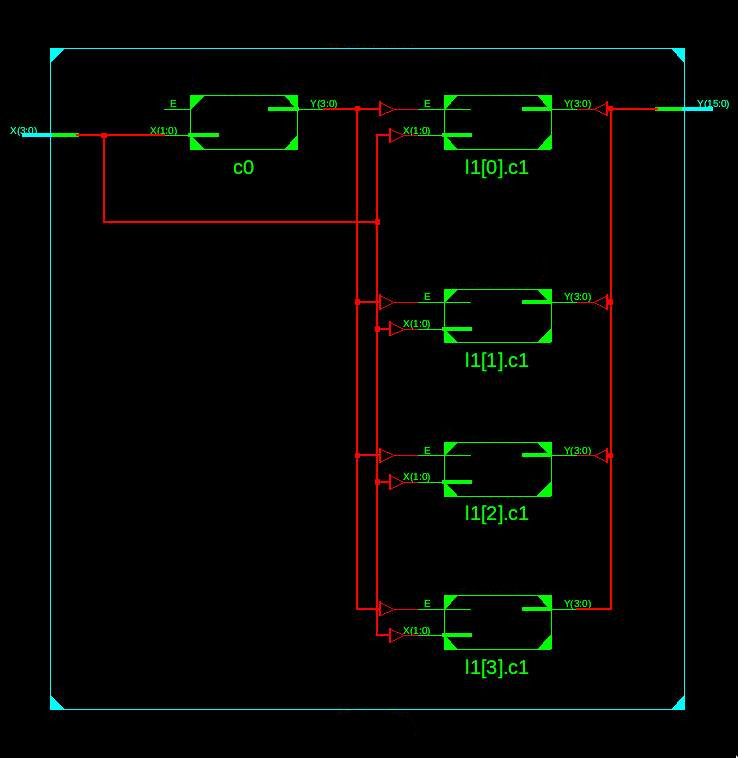
\includegraphics[width=12cm]{./figures/4x16.jpeg}
        \caption{4x16 circuit diagram}
    \end{figure}
    \section{Code}
    \subsection{Using function of 2x4 decoders only}
    \inputminted{vhdl}{./codes/ass3_annex2a.vhd}
    \subsection{Using procedures of 2x4 decoders only}
    \inputminted{vhdl}{./codes/ass3_annex2b.vhd}
    \section{Test Bench}
    \inputminted{vhdl}{./codes/tb_a3_ax1.vhd}
    \section{Timing diagram}
    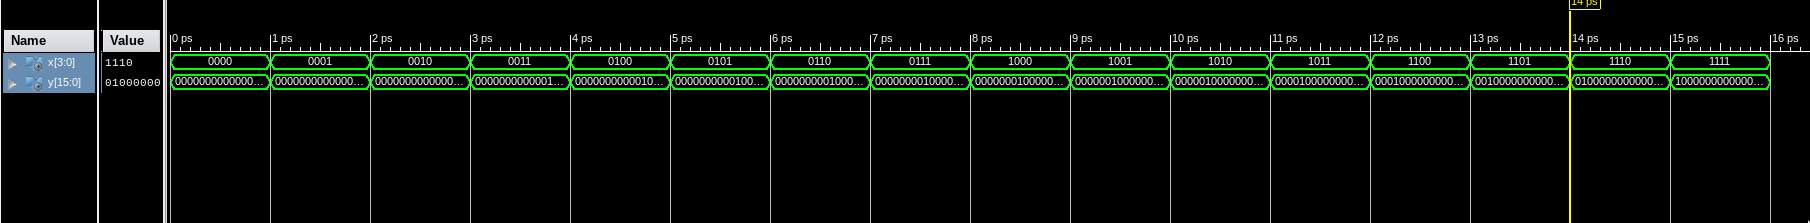
\includegraphics[width=19cm]{./figures/td_4x16.jpeg}

\end{document}
